\chapter{Architecture du projet}
\section{Gestionnaire de configuration}
\paragraph{}
Nous avons utilisé Maven pour la gestion du projet. Ce dernier prend racine sur un méta-projet servant à capitaliser les dépendances redondantes à chaque sous-projet. Nous avons développé deux sous projets Maven. L'un correspondant au front-end de l'application (client) et l'autre au back-end (service).

\section{Architecture service}
\paragraph{}
Le back-end a été développé en J2EE à l'aide de Jersey et JPA. L'architecture du service est présentée dans la figure~\ref{service}, page~\pageref{service}.

\begin{figure}[ht]
\caption{\label{service} Architecture service}
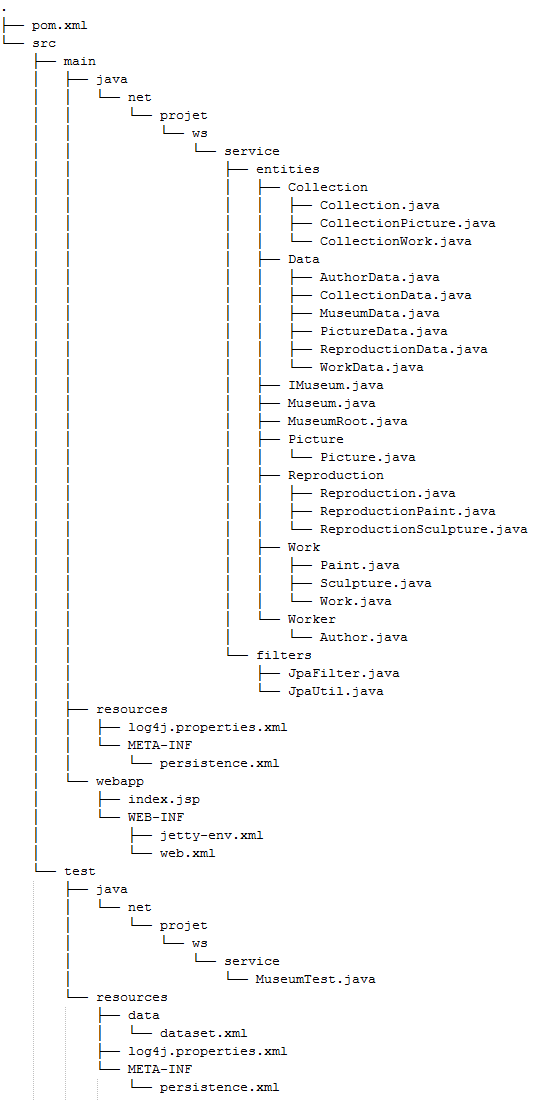
\includegraphics[scale=0.65]{service}
\end{figure}

\paragraph{}
Le dossier /entities contient toutes les classes annotées JPA qui seront traduites dans le domaine relationnel. Le fichier MuseumRoot.java contient tous les points d'accès pour les méthodes REST dans le but d'interroger la base de données. L'interrogation passe par les fichiers contenus dans le dossier Data/ ayant accès à un EntityManager instanciable via des filtres (/filters).

\paragraph{}
Une phase de test a été intégrée au cycle de Maven avant la phase de déploiement. La phase de tests:
\begin{enumerate}
\item instancie une nouvelle base de données;
\item établit une communication via un EntityManager;
\item efface et remplit la base de données à l'aide d'un fichier de données XML;
\item exécute une méthode de test;
\item répète les étapes 3 et 4 jusqu'à ce que tous les tests soient terminés;
\item envoi les résultats des tests dans des fichiers de sortie.
\end{enumerate}

\section{Architecture client}
\paragraph{}
Le client a été développé en web 2.0 avec un design MVC à l'aide du framework AngularJS. L'architecture du service est présentée dans la figure~\ref{client}, page~\pageref{client}.

\begin{figure}[ht]
\caption{\label{client} Architecture client}
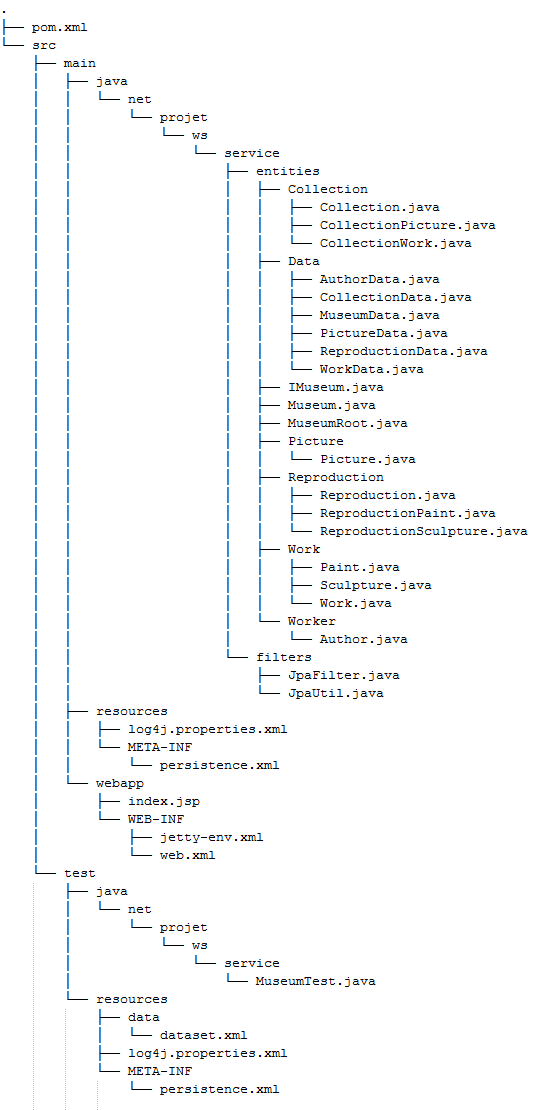
\includegraphics[scale=0.65]{client}
\end{figure}


\paragraph{}
La communication avec le service du musée passe par l'intermédiaire d'un serveur express. Ainsi, seul le serveur express dispose des chemins pour accéder et modifier les requêtes reçues~/~envoyées au serveur du musée.